%\q{1}{Combinatorics Questions}\\

\q{1}{Rolling Dice} If you roll a fair dice $n$ times:

\sq How many times will the sequence 1,2,3,4,5,6 occur?  What is the
probability of this occurring?

\sq How many times will the sum of the number of 1's and 2's equal the
sum of the number of 3's, 4's, 5's and 6's?  What is the probability
of this occurring?

\sq How many times will the sum of the number of 1's and 2's equal the
sum of the number of 3's and 4's and equal the sum of the number of
5's and 6's?  What is the probability of this occurring?

\sq How many times will you roll a 1 twice in succession?  For the
purpose of this calculation, the sequence ...11.... counts as once,
but so does ...111....  The sequence ...1111... counts as twice.  What
is the probability of this occurring?

\sq How many times will you roll a 1 $k$-times in succession?  As with
the previous case, when a 1 is counted as part of a $k$-sequence, it
is not counted as part of a subsequent $k$-sequence.  What
is the probability of this occurring?

\sq You have a communications system that transmits bundles of data
from a source to a destination.  Most bundles are received correctly.
However, there is a random chance of the data in a bundle being in
error.  Roughly every $E^{th}$ bundle is in error.  If you transmit
$n$ bundles, what is the probability of two bundles in sequence being
in error?  what is the probability of $k$ bundles in sequence being in
error?

You may wish to modify your Lab3 program {\tt dice} to give you a
sense of whether or not your answers look correct.

\q{1}{Binomial Theorem} Prove (using induction) the binomial theorem:
\[
(x+a)^n = \sum_{r=0}^n C(n‚ r)x^{n-r}a^r
\]

\newpage
\q{1}{Graph Questions} Is there

\sq a graph with 5 vertices and 3 edges?

\sq a graph with 5 odd-degree vertices with 3 edges?

\sq a connected graph with 5 vertices and 3 edges?

\sq a directed graph with 5 vertices and 3 edges?

\sq a disconnected graph (a graph that is not connected) with 5
vertices and 7 edges?

\sq a disconnected, directed graph with 5 vertices and 7 edges?

\sq a graph with 3 vertices and 5 edges?

\sq a directed graph with 3 vertices and 5 edges?

In each case, if there exists such a graph, illustrate it; if not,
explain (precisely) why not.

\newpage

\q{1}{Given a Graph} Given the following graph:

\begin{center}
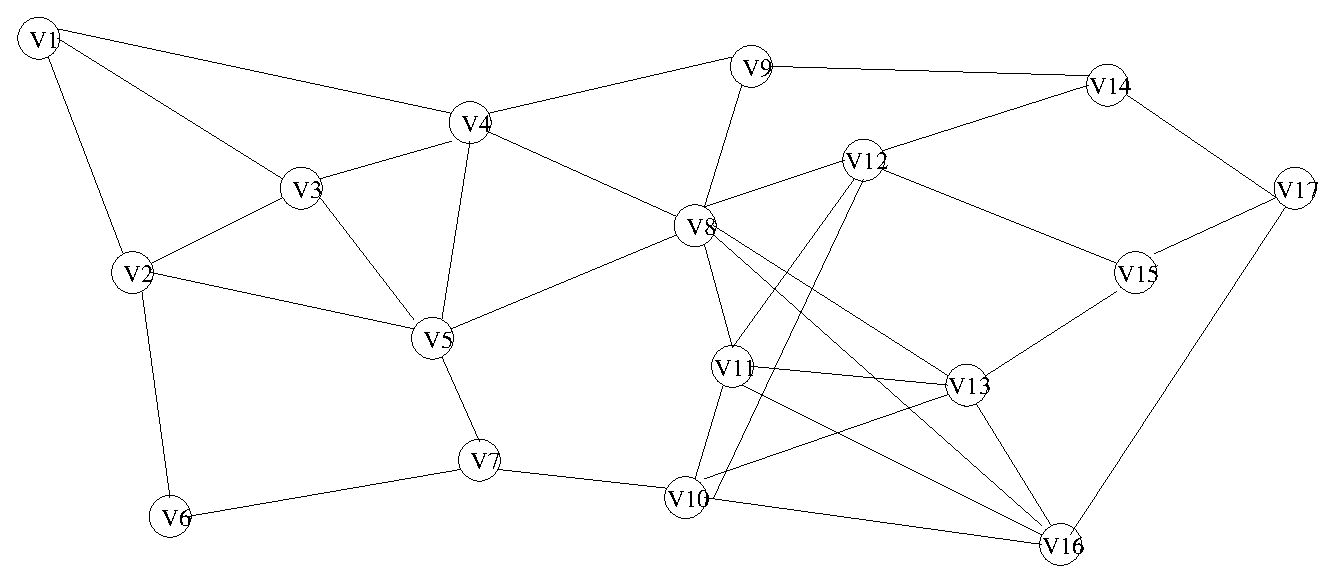
\includegraphics[scale=0.7]{Figures/graph.eps}
\end{center}

\sq Is this graph connected?

\sq Is this graph complete?  Why/Why not?

\sq What is the minimum degree of the graph?

\sq What is the maximum degree of the graph?

\sq What is the largest clique in the graph?

\sq Is the graph planar? Why/Why not?

\sq What is the shortest path from V1 to V17? How long is it?

\sq What is the longest path from V1 to V17?  How long is it?


